%% ==============================
\chapter{\iflanguage{ngerman}{Methoden}{Methods}}
\label{sec:methods}
%% ==============================


Die Implementierung dieser Arbeit orientiert sich an dem zweistufigen Clusteringverfahren aus der Arbeit von Nguyen \cite{nguyen2012clustering}.
 
Die hier vorgestellte Implementierung teilt sich in zwei verschieden Programme auf. Zum einen ein Programm, dass Volumedaten lädt, verarbteit und das Ergebnis als binäre Datei abspeichert und zum anderen ein Unityprogramm, das für die Visualisierung von den binären Volumendaten zuständig ist. 
Das Modul zum Laden und Speichern von Volumendaten, sowie das Unityprogramm zum rendern von Volumendaten sind in Vorarbeiten des IPRs entstanden und  werden in dieser Arbeit teilweise vorgestellt und verwendet. 
\todo{christians paper}

Anfangs liegen die CT-Daten von den Volumen als Schnittbilder im DICOM Format vor. Diese werden mithilfe der MITK Workbench zu einer einzelnen Datei im .nrrd Format umgewandelt, welche vom Programm eingelesen werden können.
Da CT-Daten Werte im negativen Bereich haben, die für  das Verfahren hinderlich sind, werden die Daten um den kleinsten Wert verschoben, sodass das Minimum des Volumens bei null liegt.


Zunächst müssen die LH-Werte des Volumen berechnet werden, dafür müssen die Gradienten aller Voxel bestimmt werden. Wie im Paper beschrieben wurde in dieser Arbeit auch Hong's Methode \cite{hong2003method} dafür gewählt.
Diese ist ein Approximationsbasiertes Verfahren zur Berechnung von Gradienten eines Volumens vorgestellt. 
\newline
 In Hong's Verfahren wird zur Berechnung die lokale 4x4x4 Nachbarschaft hinzugezogen. Hierbei ist zu beachten, dass der Gradient für einen Punkt nicht direkt berechnet werden kann. Der Gradient kann immer nur zwischen zwei Punkten berechnet werden, da er die Veränderung der Werte angibt. Deshalb liegt er im Falle eines dreidimensionalen Volumens im Zentrum eins Würfels, der von 8 benachbarten Voxeln aufgepsannt wird, wie man in \autoref{fig:nachbarschaft} sehen kann. Die Knoten sind hierbei die Voxel des Volumens in denen ein Intensitätswert gespeichert ist.
\newline

\begin{figure}[!h] 
\centering 
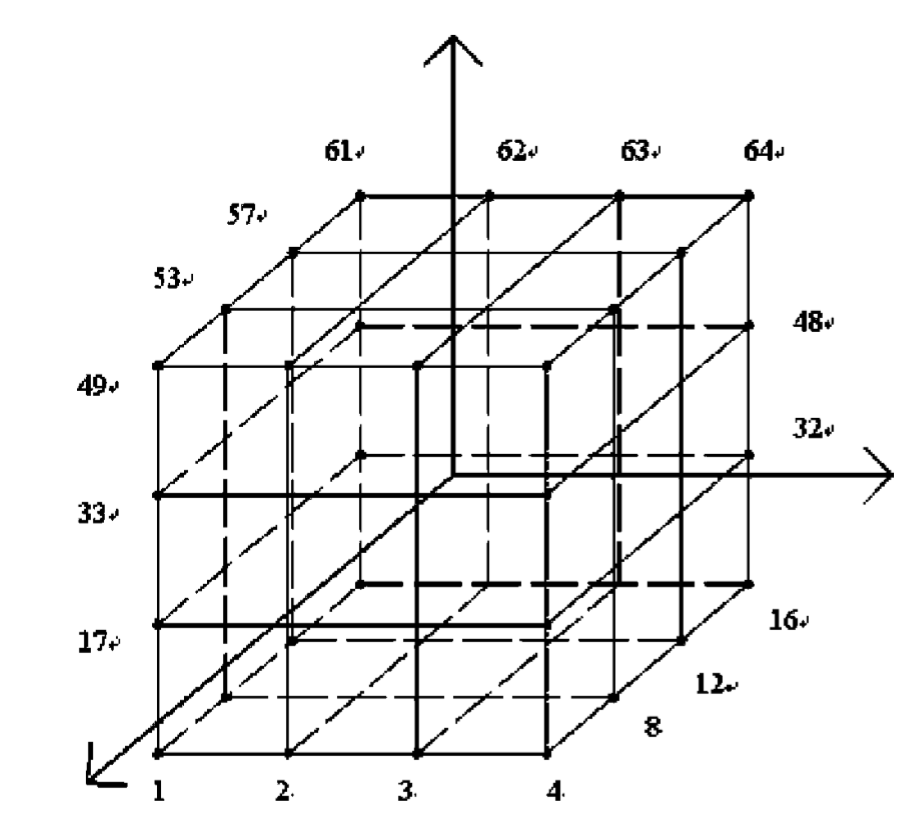
\includegraphics[width=\textwidth]{Logos/VoxelEdges.PNG}
\caption{Darstellung der lokalen 4x4x4 Nachbarschaft} 
\label{fig:nachbarschaft} 
\end{figure}
\todo{richtig bild zitieren u. evtl kleiner}




Die Funktionen für die Intensitätswerte wird im Paper mit:
\newline
$f(x,y,z) = Ax^{2}+By^{2}+Cz^{2}+2Fyz+2Gzx+2Hxy+2Ix+2Jy+2Kz+D$ 
\newline
approximiert. Da der Gradient die Ableitung der Intensitätsfunktion ist, erhält man den dreidimensionalen Gradientenvektor n, indem die Funktion ableitetet wird:
\newline
$n = (Ax+Gz+Hy+I, By+Fz+Hx+J, Cz + Fy + Gx + K)$ .
\newline
Um den Gradienten zu Berechnen müssen die Parameter A,B,C,E,F,G,H,I,J,K  berechnet werden. Dies geschieht mithilfe der Methode der kleinsten Quadrate.
\todo{methode der kleinsten quadrate genauer beschreiben}

Dies wird für jeden Voxel im Volumen berechnet. Als Ergebnis des Verfahrens kommt ein Volumen, in dem alle Gradienten gespeichert sind, heraus. Jedoch sind die Punkte um eine halbe Voxellänge verschoben. Desweiteren ist die Dimension dieses Volumens in jeder Achse um eins kleiner als das vorher gegebene Intensitätsvolumen.
Da für die Berechnung der LH-Werte jedoch der Gradient und der Intensitätswert an einer Stelle im Volumen bekannt sein muss, wurden die Intensitätwerte auf das Volumen der Gradienten umgerechenet. Dies geschieht durch eine einfach Interpolation indem von allen 8 Nachbarn eines Punktes der Intensitätwert geachtelt wurde und aufaddiert. Hierbei gehen Information verloren....
\todo{abbildung für interpolation und beschreiben was verloren geht}


Nachdem die Gradienten berechnet sind und die Intensitätswerte passend umgerechnet wurde, folgt die Berechnung der Low- und High-Werte. Dazu wird in Richtung der Gradienten integriert. Hierfür wurde wie von Nguyen auch Heun's Methode, eine modifizierte Euler Methode verwendet. Die hierzu benutzte Formel lautet:
\newline
$u_{i+1} = u_{i} + \frac{1}{2}d(\triangledown f (u_{i}) + \triangledown f(u_{i}+d \triangledown f(u_{i}))) $
\newline
Hierbei sind $u_{i}$ und $u_{i+1}$ die Positionen des aktuellen, beziehungsweise des nächsten Voxels. $\triangledown f(x)$ beschreibt den normalisierten Gradienten für die High-Werte und den normalisierten inversen Gradienten für die Low-Werte an Stelle $x$ . $d$ steht für die Schrittweite (ein Voxel).
Da das Verfahren in dieser Arbeit auf CT-Daten angewendet wird, ist das Abbruchkriterum der Integration, dass ein Gradient mit Länge null gefunden wird. Ist dies der Fall wir der Intensitätswert dieses Voxels als Ergebnis für den Low- beziehungsweise High-Wert des Startvoxel festgelegt.


Anschließend wird ein LH-Histogram über alle berechneten Werte erstellt. Die x-Achse sind hierbei die Low- und die y-Achse die High-Werte. Deren Reichweite geht von null bis zu den jeweiligen Maxima der Werte.

Auf diesem Histogram findet der erste Clusteringschritt  statt. Es wird ein Meanshiftclustering verwendet. Dazu wird zuerst eine Bandweite und ein Threshold gewählt, welche die Sensitivität des Clusterings bestimmen. Danach wird das Clustering für jeden Punkt im LH-Histogramm wie folgt durchgeführt.
\newline
Es werden alle Punkte die innerhalb des Radius der Bandbreite um den Startpunkt liegen gespeichert. Diese Punkte bilden nun den gefundenen Cluster. Von diesem Cluster wird der neue Mittelpunkt, der jeweilige Mittelwert der beiden Koordinaten, berechnet. Um diesen Punkt wird erneut mit selben Radius alle Punkte die bisher nicht zu dem Cluster gehören gesucht und hinzugefügt. Dies geschieht solange, bis der Abstand des neu kalkulierte Mittelpunkt zum Alten weniger als der Threshold mal die Bandweite ist. 
Nachdem das Clustering für jeden Punkt im Histogramm beendet ist, werden jene Cluster deren Mittelpunkte eine Distanz kleiner als die Hälfte der Bandweite zueinander haben miteinander zu einem einzigen Cluster verschmolzen.


\todo{intensitätswert ventrikel, vllt orginial werte nehmen und in implementierung verschiebun vorstellen}
Da die Intensitätswerte im Gehirn sehr nah beieinander liegen, wäre es nicht sinnvoll wie von Nguyen beschrieben über das komplette Histogramm mit einer Bandweite von 7\% - 9\% des maximalen LH-Wertes, das Maximum aller Low- und High-Werte, zu clustern. Das Gehirn würde dabei als ein paar wenige, sehr große Cluster erkannt werden. Diese Herangehensweise mag praktibale zum Darstellen von Knochen, des kompletter Gehirns oder anderen Bereiche sein, entspricht jedoch nicht dem Ziel dieser Arbeit, das Ventrikelsystem kenntlich zu machen und zu visualisieren. Aus diesem Grund wurde die Bandbreite des Clustering auf 0,1\% des maximalen LH-Wertes gesetzt. Da so eine Bandbreite sehr Rechenaufwendig ist und bekannt ist, dass das Ventrikelsystem einen Intensitätswert um die ... hat, wurde desweiteren nur im Intensitätswertbereich von 1025 bis 1075 geclustert, um die Rechenzeiten gering zu halten.Weiterhin wurde nicht jeder Punkt des Histograms besucht, sondern eine Schrittweite von fünf Kasten festegelegt. Dies geschah aus der Beobachtung heraus, dass für zwei oder drei direkt nebeneinanderliegende Kasten im LH-Histogramm meist der gleiche Cluster als Ergebnis berechnet wurde. Diese wurden im letzten Schritt dann ohnehin zu einem einzigen Cluster verschmolzen, was die Berechnung jedes einzelnen Kastens unnötig machte. Diese Maßnahmen dienen ausschließlich dem Zweck Strukturen im Gehirn bessers unterscheiden zu können, da sie so in verschiedne LH-Cluster eingeteilt werden und damit unterscheidbar sind. Wenn das Verfahren für andere Ziele genutzt werden soll, können die Parameter auf die von Nguyen vorgeschlagenen Werte gesetzt werden. 

\todo{allgemein meanschiftclustering beschreiben}



Als nächstes werden die LH-Cluster erneut mit Meanshiftclustering geclustert. Diesmal jedoch anhand ihrer räumlichen Informationen im Volumen. Im Paper von Ngujen wird hierzu kein Wert für die Bandbreite vorgeschlagen. In dieser Arbeit hat sich eine Bandbreit von 10  und eine minimale Distanz vom alten zum neuen Mittelpunkt von 0,01 als zielführend erwiesen.



Nachdem alle Cluster erzeugt wurden, werden ihnen zufällige IDs von eins bis zur Anzahl an Clustern zugeteilt. Anschließend wird ein Volumen erstellt, mit den Dimensionen des ursprünglichen Intensitätsvolumens, dass nur mit nullen als Werte gefüllt ist. Warum es diese Dimension haben muss, wird später erklärt. Danach wird durch alle Cluster iteriert, und jeder Voxel in das neu erstellte Volumen an der jeweiligen Position eingetragen. Dabei ist der eingetragene Wert immer die  ID des aktuellen Clusters. Nachdem alle Cluster abgearbeitet wurden, besteht das Volumen aus ausschließlich nullen und den IDs der Cluster an den passenden Stellen.


Dieses Volumen wird als eine binäre Datei abgespeichert und in Unity geladen. Hier kann der Anwender sich entweder die Form von einzelnen IDs anschauen oder eine Reichweite von IDs. Die gewählten IDs werden rot markiert und sich deutlich vom restlichen Volumen zu unterscheiden. Mithile der Darstellung muss der Nutzer anhand der Form die Cluster erkennen, die zum Ventrikelsystem gehören, und deren IDs notieren. 

Hat er dies getan kann er im ... Programm die binäre Datei mit den IDs, die ursprüngliche Intensitätsvolumendatei laden und eine die Liste der passenden IDs als Parameter übergeben. Die ausgewählten IDs werden zu einem Cluster gemerged und in das Intensitätsvolumen übernommen. Dort erhalten sie, da der maximale Wert von CT-Daten bei ...(4400) liegt, den Wert 5000. Dieser Wert erhöht das Maximum für die Darstellung der Daten nur gering, ist dafür aber im Volumen sonst niergends enthalten. Das Ergebnis dieses Merges wird wieder als binäre Datei gespeichert.

Als letzten Schritt kann nun der Benutzer die gemerged Datei erneut in Unity laden. Hier kann er sich dann das Volumen normale abhängig von den Grauwerten dargestellt anzeigen lassen, mit dem Ventrikelsystem in rot, oder einer anderen ausgewählten Farbe darin.

\todo{letzten schritt genauer}

